\section{Lenguajes de Descripción de Arquitectura}

\subsection{La necesidad de una arquitectura de referencia}

La necesidad de una arquitectura de referencia, o arquitectura objetivo; es una parte esencial dentro de la computación autonómica. Esta forma parte de la base de conocimiento (K), y, de manera indirecta, de los objetivos del administrador del sistema \cite[p. 24]{lalanda_diaconescu_mccann_2014}. 

Con el fin de fijar un objetivo para nuestro sistema autonómico, fue necesario determinar una manera de realizar la declaración de dicha arquitectura, que estableciera un estado de referencia. De esta manera, podría evaluarse el estado del sistema en tiempo de ejecución,  y así tomar las acciones necesarias para adaptarlo hacia el estado de referencia. 

% \subsection{La noción de aplicación}

Ahora, es necesario establecer el punto desde el cual se realizará la comparación entre los estados del sistema. Esto guiará la búsqueda para determinar el como se realizará la declaración de los estados objetivo de Smart Campus UIS, al igual que los datos que se recolectarán.

Siendo así, y dados los objetivos que buscan cumplir los ecosistemas inteligentes para la toma de decisiones \cite{Anagnostopoulos_2023}, se estableció que la métrica por la cual se describiría, y evaluaría, el estado del sistema sería a partir de los datos que estaban siendo recolectados. Es decir, que nuestro enfoque debía estar orientado a cumplir con las necesidades de los datos establecidas por Smart Campus. 

\subsection{Criterios de selección}

Con el fin de establecer la notación a usar para la declaración de las arquitecturas objetivo, se establecieron unos lineamientos con los cuales se realizaría la evaluación de las diferentes notaciones ya desarrolladas anteriormente. De esta manera se podría escoger la manera a representar los modelos, o en el caso de ser necesario, establecer los criterios por el cual se podría desarrollar uno.

En la tabla \ref{tab:criterios}, se presentan los criterios usados para la selección, con su respectiva explicación y valor considerado para la selección.

\begin{table}[H]
    \centering
    \vspace{-4mm}
    \caption{Criterios usados para la determinación de la notación a utilizar} \label{tab:criterios}
    \vspace{4mm}
    \begin{tabular}{lm{4.7cm}m{0.51\linewidth}c}
        \hline
        \multicolumn{1}{l}{} &
        \multicolumn{1}{c}{\textbf{Criterio}} &
        \multicolumn{1}{c}{\textbf{Explicación}} &
        \multicolumn{1}{c}{\textbf{Valor}} \\ \hline
        C1 & \centering Describir la arquitectura de un sistema IoT &
        Este criterio es una base a establecer con el fin de descartar aquellos lenguajes de notación generales o no necesariamente usados para la descripción de arquitecturas IoT. &
        Alto \\ 
        C2 & \centering  Permitir la especificación de la ubicación del componente &
        La especificación de la ubicación de los componentes es importante en los sistemas IoT, especialmente dentro del contexto del proyecto en el cual se está trabajando con un Smart Campus; ya que los componentes pueden estar distribuidos en diferentes ubicaciones físicas y la evaluación de su integridad puede depender de su presencia en un lugar dado. &
        Alto \\ 
        C3 & \centering Habilitar el modelado del componente a nivel de sus entradas &
        Es importante poder describir las entradas de los componentes, específicamente los datos que manejan, así como su rol dentro del sistema. &
        Alto \\ 
        C4 & \centering Modelar el comportamiento de los componentes &
        La notación debe permitir modelar el comportamiento de los componentes, de manera que se puedan entender sus interacciones y su función en el sistema IoT. Dentro del contexto del proyecto, no es tan relevante, ya que no se está evaluando la funcionalidad del sistema, sin embargo, para futuros trabajos, podría facilitar la extensión de Smart Campus UIS. &
        Bajo \\ 
        C5 & \centering Posibilitar el establecer los estados de los componentes &
        La notación debe poder definir los estados de los componentes. Estos estados pueden ser tanto de comportamiento o operacionales. &
        Medio \\ 
        C6 & \centering Permitir de exportar el modelo descrito a gráficas u otros formatos &
        Es importante que la herramienta permita exportar el modelo descrito en diferentes formatos para facilitar su integración con otras herramientas y sistemas, y para permitir su visualización en diferentes formatos. &
        Medio \\ \hline
    \end{tabular}
    \vspace{-4mm}
\end{table} 

\subsection{Búsqueda de Alternativas}

Una vez establecidos los criterios de selección, se realizó una exhaustiva búsqueda de alternativas disponibles en la literatura y en la industria para describir arquitecturas para describir la arquitectura de sistemas IoT. Esta búsqueda se realizó a partir de la revisión en diferentes bases de datos, como \textit{Scopus}; al igual que algunas de las revistas especializadas en el tema, y el internet en general.

Durante la búsqueda, se identificaron una gran variedad de opciones. Sin embargo, la gran mayoría de estos se filtraron, o descartaron; a partir de los criterios de selección establecidos. Esto se debe a que los LDAs usados en la tanto en la industria y academia, como AADL (Architecture Analysis and Design Language), tienen un enfoque a los campos de aviónica, equipos médicos y aeronáutica (lo que complicaría su implementación hacia sistemas de software IoT) \cite{aadl_web, aadl_pdf}; o SysML, que son demasiado genéricos y abarcan hardware, software e incluso personas y procesos \cite{omgsysml_2015}.

Entonces, de las posibles opciones de notación, se seleccionaron cinco las cuales fueron evaluadas con el fin de determinar si alguna de las opciones hubiera podido ser usada, o si era necesario desarrollar nuestra propia notación. A continuación, se presentan las alternativas evaluadas:

\begin{itemize}
    \item \textbf{MontiThings:} Basado en MontiArc, otro LDA más general; está diseñado para el modelado y prototipado de aplicaciones de IoT. Este realiza las descripciones de sus arquitecturas en un modelo componente-conector, donde los componentes están compuestos por otros componentes; y los conectores definen la manera en la que se comunican estos componentes a nivel de los datos y la dirección de estos. \cite{MontiThings, MontiThingsRepo}
    \item \textbf{Eclipse Mita}: Mita, creado por la Eclipse Foundation; es un lenguaje de programación orientado al facilitar la programación de sistemas IoT. Aunque como tal no es un LDA, está orientada a la descripción de los componentes y el comportamiento del sistema establecido, de esta manera, puede generar el código que debe correr en los dispositivos embebidos \cite{Mita}. 
    \item \textbf{SysML4IoT:} Es un perfil de SysML\footnote{Los perfiles se refieren a extensiones a UML, en este caso es una extensión de SysML en sí \cite{Charles2007}.} en la cual se usan estereotipos de UML con el fin de abstraer las diferentes partes de los sistemas de IoT. Al igual que SysML, este permite el modelado más allá de dispositivos incluso llegando a personas y procesos, con la diferencia del enfoque dado al \textit{dominio de IoT} \footnote{El \textit{dominio del IoT}, hace referencia al \textit{Architecture Reference Model} establecido por IoT-A, un consorcio Europeo el cual buscaba el establecer un modelo para la interoperatividad de dispositivos IoT. \cite{IoTA2014}} \cite{SysML4IoT2016}.
    \item \textbf{ThingML:} Similar a Mita, ThingML, es un lenguaje de modelado el cual tiene capacidades de generar el código requerido por los dispositivos embebidos. En términos del proyecto, este permite el modelado de los sistemas de IoT a partir de \textit{state machine models}\footnote{Los \textit{state machine model}, también conocidas como Autómatas Finitos; son modelos matemáticos que describen todos los posibles estados de un sistema a partir de unas entradas dadas \cite{StateMachine2023}. } los cuales permiten describir los componentes del sistema al igual que el comportamiento de estos \cite{ThingML2016}.
    \item \textbf{IoT-DDL}: Iot-DDL es un LDA, implementado en XML, que describe objetos dentro de los ecosistemas IoT con base en sus componentes, identidad y servicios entre otros. Este tiene la capacidad de describir parte de la base de conocimiento que tienen los diferentes componentes (Principalmente relaciones y asociaciones entre componentes) \cite{Ahmed2018}.
\end{itemize}

Una vez seleccionadas las alternativas a evaluar, se utilizó la matriz de evaluación en la tabla \ref{tab:evaluation} para determinar la solución ideal para el desarrollo del proyecto. 

\skipline
\skipline
\skipline
\skipline

\begin{table}[H]
    \centering
    \vspace{-4mm}
    \caption{Evaluación de las alternativas en función de los criterios establecidos} \label{tab:evaluation}
    \vspace{4mm}
    \begin{tabular}{cccccc}
    \hline
    \multicolumn{1}{l}{} &
      \multicolumn{1}{l}{MontiThings} &
      \multicolumn{1}{l}{Eclipse Mita} &
      \multicolumn{1}{l}{SysML4IoT} &
      \multicolumn{1}{l}{ThingML} &
      \multicolumn{1}{l}{IoT-DDL} \\ \hline
      C1 & ✓ & ✓ & ✓ & ✓ & ✓ \\
      C2 & ✗ & ✗ & ✗ & ✗ & ✗ \\
      C3 & ✓ & ✓ & ✓ & ✓ & ✓ \\
      C4 & ✓ & ✓ & ✓ & ✓ & ✗ \\
      C5 & ✓ & ✓ & ✗ & ✓ & ✗ \\
      C6 & ✗ & ✗ & ✗ & ✓ & ✗ \\ \hline
    \end{tabular}
    \vspace{-4mm}
\end{table}

Partiendo de los resultados de la evaluación, se puede apreciar que ninguno de estos LDA cumple con los criterios establecidos para el proyecto. Aunque estos están orientados hacia la descripción y desarrollo de sistemas IoT, no están enfocados hacia su contexto en términos de aplicación más allá de la definición de comportamiento. Esto se debe a los objetivos de cada una de estas notaciones, de una u otra manera; buscan el representar como tal el sistema IoT en términos de su funcionalidad técnica y no la aplicación en si. 

\subsection{Un nuevo modelo para Smart Campus}

Dado que no hay una alternativa que se adapte completamente a las necesidades del proyecto, se tuvo que definir nuestro propia notación la cual permita modelar las arquitecturas a nivel de aplicación bajo el contexto de un Smart Campus, tomando en cuenta los criterios definidos como guía para el desarrollo.

Primeramente, fue necesario que definir un metamodelo el cual permita establecer la manera en la que se verán estas arquitecturas. Para ello, y partiendo de la implementación a realizar, nos basamos parcialmente en el modelo establecido por \citeA[p. 63]{msc_henry_2022}. 

\begin{figure}[H]
    \centering
    \caption{Versión 2 del modelo concepto planteado por}
    \citeA[p. 63]{msc_henry_2022}
    \label{fig:henrymodelo}
    \vspace{2mm}

    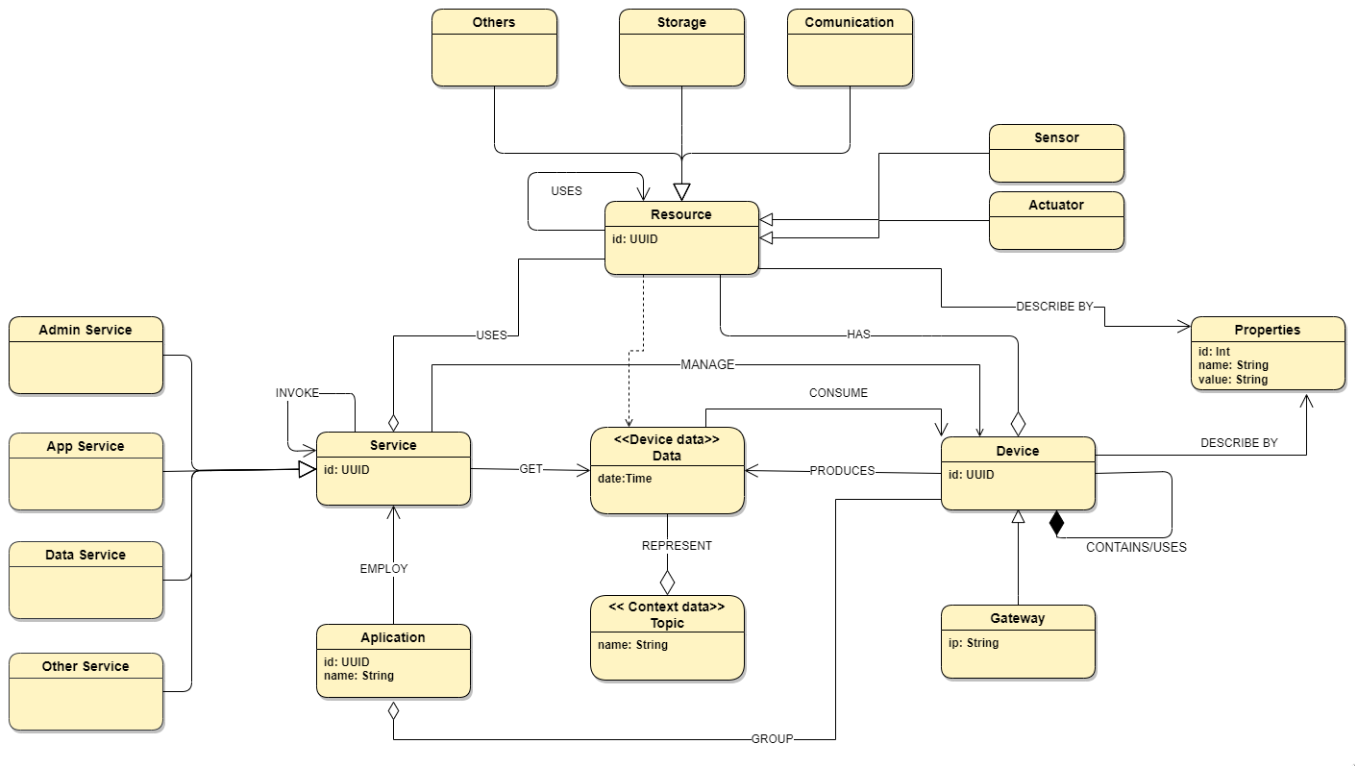
\includegraphics[width=\linewidth]{images/Henrymodelo.png}
\end{figure}

% En este modelo, se presentan todas los componentes que componen a Smart Campus UIS en términos de su arquitectura a un nivel técnico. Ahora, para modelar un Smart Campus a nivel de aplicación, se tomó una versión reducida de este modelo enfocándose en los componentes y a la función que estos cumplen en una ubicación geográfica dada. 

% El basarnos en este modelo nos asegura que se tiene la capacidad de realizar la descripción de un un sistema IoT de Smart Campus en un nivel técnico. Este contiene todos los componentes necesarios para poder modelar

Basarnos en el modelo de la figura \ref{fig:henrymodelo}, nos da la capacidad de describir a un nivel técnico un sistema IoT. Ahora, aunque se podría usar para el desarrollo del proyecto, fue necesario modificarlo con el fin de acercarnos más hacia la descripción de un sistema IoT a nivel de aplicación. 

Lo primero fue el establecer el contexto de los dispositivos. Esto específicamente se refiere al criterio \textit{C2} de la tabla \ref{tab:criterios}, en donde, dada la necesidad de establecer la ubicación geográfica en algunas de las aplicaciones de los Smart Campus, era necesario poder describir los lugares pertenecientes a la aplicación.

Así mismo, se cubre el criterio \textit{C3} cambiando las propiedades del dispositivos de una clase, externa a los dispositivos; a un atributo, interno, el cual le permite a los componentes manejar su propia información en cuanto a los datos que estos manejan. Estas propiedades puede referirse a las entradas que tienen, en el caso de ser actuadores o procesadores de la información; o a los valores que reportan al sistema en el caso de ser sensores.

Partiendo de esto, se planteó el modelo presente en la figura \ref{fig:metamodelo}.

\begin{figure}[H]
    \centering
    \caption{Versión 1 del metamodelo planteado para SCampusADL}
    \label{fig:metamodelo}
    \vspace{2mm}
    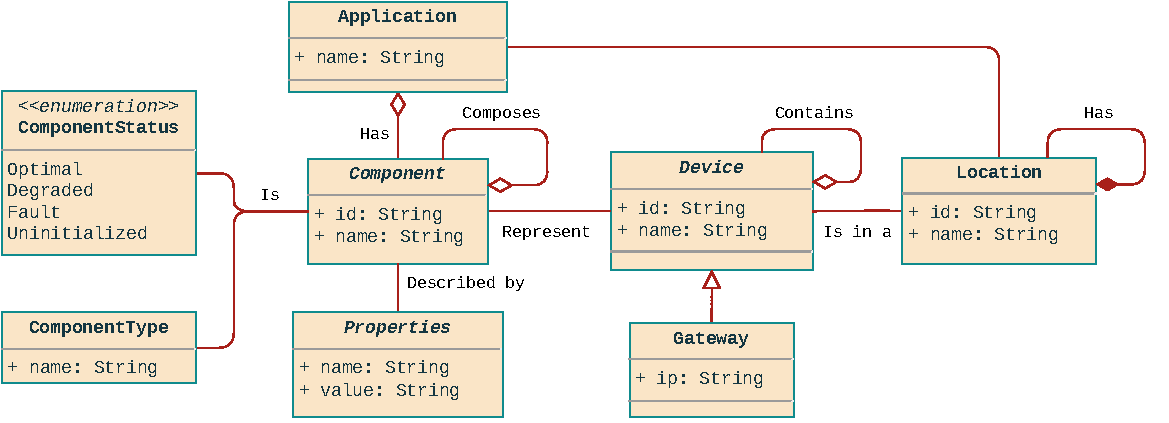
\includegraphics[width=0.8\linewidth]{images/Metamodel B.pdf}
\end{figure}

El enfoque principal del modelo se centra los componentes (\texttt{\textit{Component}}). Estos son las representaciones lógicas, o de software, de las partes de la aplicación. De manera general, pueden ser tanto servicios usados por la aplicación como agregadores de datos, pre-procesadores de datos encargados de transformar los datos recolectados, o incluso los mismos sensores o actuadores que hacen parte del sistema (\textit{\texttt{componentType}}). 

Los componentes pueden ser atómicos, funcionando como entidades independientes, o formar parte de componentes, así como integrarse en componentes aún más grandes. Asimismo, los componentes se describen por una serie de propiedades que hacen referencia tanto al comportamiento al igual que las condiciones las con las cuales se puede evaluar el estado del mismo. 

Estos elementos están presentes en diversos dispositivos (\texttt{\textit{Device}}), los cuales se encargan de la ejecución de partes de la aplicación, o puntos de comunicación entre diversos componentes (\textit{\texttt{Gateway}}). Estos pueden verse como los recursos físicos de la aplicación los cuales se encuentran ubicados en diferentes puntos, o locaciones (\textit{\texttt{location}}), dentro del Campus (\textit{\texttt{Campus}}). 

Lo anterior nombrado hace parte del contexto de la aplicación. Siendo así, estos están relacionados contra la aplicación la cual sirve como un punto de acceso común entre el contexto geográfico y los componentes de software que deben ser manejados.

Finalmente, los estados de los componentes (\textit{\texttt{ComponentStatus}}), reflejan el como estos se encuentran dentro del contexto de la aplicación. Estos pueden variar de óptimo (\textit{\texttt{optimal}}), donde todos los componentes están funcionales según las propiedades establecidas; degradado (\textit{\texttt{degraded}}), donde uno o más de los componentes opcionales está fallado; y fallo (\textit{\texttt{fault}}), que es cuando alguno de los dispositivos obligatorios no está en funcionamiento.

\subsection{Sintaxis de la notación}

Partiendo de esto, lo siguiente que se realizó fue la definición de la sintaxis de la notación a usar, basados en lo definido por el metamodelo. Para esto, se decidió a usar \texttt{YAML}, un lenguaje de serialización de datos orientado a la legibilidad, reconocido y usado principalmente para la creación de archivos de configuración \cite{YAML2023}. 

La sintaxis, como puede observarse en la figura \ref{fig:rail-base}, se compone de 2 partes: \texttt{locaciones}, para establecer el contexto geográfico de la aplicación; y \texttt{componentes}, con el cual se definen las partes de la aplicación al igual que las propiedades y lugar en el cual deben estar para el funcionamiento de la aplicación.

\begin{figure}[H]
    \centering
    \caption{Diagrama de rail de la sintaxis definida para la notación de SmartCampusADL}
    \label{fig:rail-base}
    \vspace{2mm}
    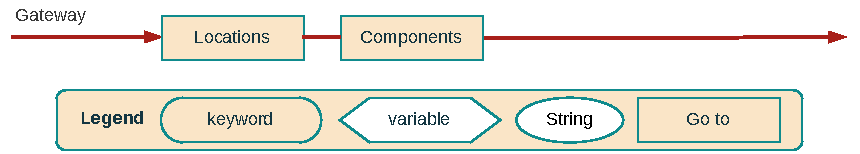
\includegraphics[width=\linewidth]{images/Railroad Base.pdf}
\end{figure}

Para especificar las \texttt{locaciones} dentro del contexto de la aplicación, se definió la sintaxis que puede observarse en la figura \ref{fig:rail-location}. De esta manera, tras especificar la \textit{keyword} \texttt{locations}, se pueden los puntos geográficos necesarios, al igual que las locaciones que lo componen. Así mismo, es posible declarar de manera implícita la ip de la \textit{gateway} que se encuentra en el lugar con el fin de poder establecer el origen de los datos recolectados. 

\begin{figure}[H]
    \centering
    \caption{Diagrama de rail de la sintaxis definida para la notación del contexto geográfico de la aplicación}
    \label{fig:rail-location}
    \vspace{2mm}
    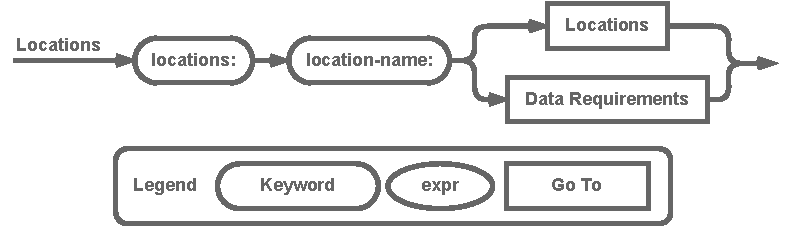
\includegraphics[width=0.8\linewidth]{images/Railroad Locations Alt.pdf}
\end{figure}

Un enfoque similar se aplicó a los componentes. En la figura \ref{fig:rail-components} se presenta la sintaxis a usar para poder definir y ubicar los componentes dentro de la aplicación. De esta forma, se pueden declarar los componentes, al igual que sus propiedades; y algunas de las características que estos deben cumplir para poder ser evaluados dentro del contexto de la aplicación.

\begin{figure}[H]
    \centering
    \caption{Diagrama de rail de la sintaxis definida para la notación de los componentes de la aplicación}
    \label{fig:rail-components}
    \vspace{2mm}
    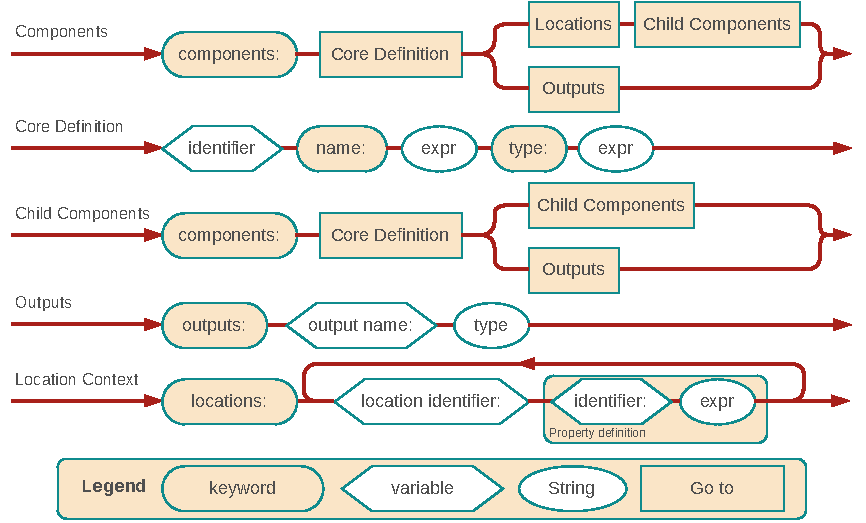
\includegraphics[width=0.8\linewidth]{images/Railroad Components Alt.pdf}
\end{figure}

Al definir esta notación, hemos creado un marco sólido para representar las aplicaciones de Smart Campus UIS. Este enfoque bien definido nos permitirá avanzar en el desarrollo de nuestras funcionalidades de comparación de los modelos, y la implementación de los mecanismos de adaptación a usar. Un ejemplo de como se vería un archivo de notación válido para nuestras necesidades puede encontrarse en el anexo \ref{appendix:example}. 

\subsection{Implementando Una Validación}

Teniendo definida la notación a usar para la declaración de las arquitecturas objetivo, lo siguiente a realizar era un módulo el cual se encargara de la validación, y construcción, los modelos a usar como referencia. La implementación, se dividió en dos partes. Una librería, la cual contiene toda la definición de los objetos definidos en el metamodelo, y será utilizada para la construcción de los modelos en todo el proyecto. La otra parte es un módulo de validación, que se encargará de verificar que los modelos definidos en la notación sean válidos de acuerdo con las reglas establecidas en el metamodelo.

La librería, apodada \textit{StarDuck}, incluye clases para representar los componentes, dispositivos, gateways, locaciones y el contexto de la aplicación. Cada clase tiene atributos y métodos que permiten establecer y acceder a sus propiedades de acuerdo con el metamodelo. Por ejemplo, la clase \texttt{Component} tiene atributos como \texttt{name} (nombre del componente), \texttt{component\_type} (tipo de componente), \texttt{components} (componentes internos), \texttt{properties} (propiedades del componente), y \texttt{outputs} (salidas del componente).

El módulo de validación, apodado \textit{Lexical}, se encarga de verificar que los modelos definidos en la notación sigan las reglas establecidas en el metamodelo. Esto incluye verificar que se definan las locaciones y componentes de acuerdo con la estructura del metamodelo, que las propiedades de los componentes sean válidas.

Para implementar la validación, se \textit{parsea} el archivo YAML y se construye una estructura de objetos de acuerdo con las clases definidas en la librería. Durante esta construcción, se aplican las reglas de validación. Si se encuentra algún error, se genera un mensaje de error indicando la ubicación del problema en el archivo de notación. En la figura \ref{fig:LexicalFlow} se puede observar un diagrama de flujo simplificado de este proceso.

\begin{figure}[H]
    \centering
    \caption{Diagrama de flujo del proceso realizado por el módulo \textit{Lexical}}
    \label{fig:LexicalFlow}
    \vspace{2mm}
    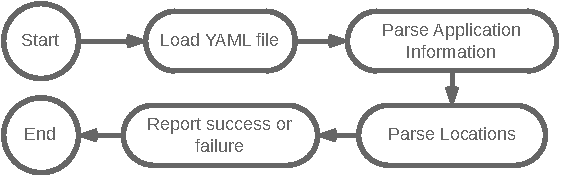
\includegraphics[width=0.8\linewidth]{images/LexicalFlow.pdf}
\end{figure}

El desarrollo de estos módulos, se realizó en Rust. Escogido debido a su capacidad para garantizar la integridad de los datos y prevenir errores comunes, lo que es esencial en un entorno donde la precisión y la confiabilidad son críticas. Además, su ecosistema de herramientas y bibliotecas facilita la implementación eficiente de los módulos de validación y construcción de modelos. \footnote{Todo el código realizado para el proyecto puede encontrase en el grupo de github \url{https://github.com/ChipDepot/}}

Con la implementación de este módulo de validación, hemos completado la primera fase del desarrollo de nuestra notación y herramienta para describir y validar arquitecturas de aplicaciones de Smart Campus. Ahora podemos avanzar en la implementación de las funcionalidades de comparación y adaptación de modelos, que son parte fundamental de nuestro enfoque de computación autonómica.


